\documentclass[twoside]{book}

% Packages required by doxygen
\usepackage{fixltx2e}
\usepackage{calc}
\usepackage{doxygen}
\usepackage[export]{adjustbox} % also loads graphicx
\usepackage{graphicx}
\usepackage[utf8]{inputenc}
\usepackage{makeidx}
\usepackage{multicol}
\usepackage{multirow}
\PassOptionsToPackage{warn}{textcomp}
\usepackage{textcomp}
\usepackage[nointegrals]{wasysym}
\usepackage[table]{xcolor}

% Font selection
\usepackage[T1]{fontenc}
\usepackage[scaled=.90]{helvet}
\usepackage{courier}
\usepackage{amssymb}
\usepackage{sectsty}
\renewcommand{\familydefault}{\sfdefault}
\allsectionsfont{%
  \fontseries{bc}\selectfont%
  \color{darkgray}%
}
\renewcommand{\DoxyLabelFont}{%
  \fontseries{bc}\selectfont%
  \color{darkgray}%
}
\newcommand{\+}{\discretionary{\mbox{\scriptsize$\hookleftarrow$}}{}{}}

% Page & text layout
\usepackage{geometry}
\geometry{%
  a4paper,%
  top=2.5cm,%
  bottom=2.5cm,%
  left=2.5cm,%
  right=2.5cm%
}
\tolerance=750
\hfuzz=15pt
\hbadness=750
\setlength{\emergencystretch}{15pt}
\setlength{\parindent}{0cm}
\setlength{\parskip}{3ex plus 2ex minus 2ex}
\makeatletter
\renewcommand{\paragraph}{%
  \@startsection{paragraph}{4}{0ex}{-1.0ex}{1.0ex}{%
    \normalfont\normalsize\bfseries\SS@parafont%
  }%
}
\renewcommand{\subparagraph}{%
  \@startsection{subparagraph}{5}{0ex}{-1.0ex}{1.0ex}{%
    \normalfont\normalsize\bfseries\SS@subparafont%
  }%
}
\makeatother

% Headers & footers
\usepackage{fancyhdr}
\pagestyle{fancyplain}
\fancyhead[LE]{\fancyplain{}{\bfseries\thepage}}
\fancyhead[CE]{\fancyplain{}{}}
\fancyhead[RE]{\fancyplain{}{\bfseries\leftmark}}
\fancyhead[LO]{\fancyplain{}{\bfseries\rightmark}}
\fancyhead[CO]{\fancyplain{}{}}
\fancyhead[RO]{\fancyplain{}{\bfseries\thepage}}
\fancyfoot[LE]{\fancyplain{}{}}
\fancyfoot[CE]{\fancyplain{}{}}
\fancyfoot[RE]{\fancyplain{}{\bfseries\scriptsize Generated by Doxygen }}
\fancyfoot[LO]{\fancyplain{}{\bfseries\scriptsize Generated by Doxygen }}
\fancyfoot[CO]{\fancyplain{}{}}
\fancyfoot[RO]{\fancyplain{}{}}
\renewcommand{\footrulewidth}{0.4pt}
\renewcommand{\chaptermark}[1]{%
  \markboth{#1}{}%
}
\renewcommand{\sectionmark}[1]{%
  \markright{\thesection\ #1}%
}

% Indices & bibliography
\usepackage{natbib}
\usepackage[titles]{tocloft}
\setcounter{tocdepth}{3}
\setcounter{secnumdepth}{5}
\makeindex

% Hyperlinks (required, but should be loaded last)
\usepackage{ifpdf}
\ifpdf
  \usepackage[pdftex,pagebackref=true]{hyperref}
\else
  \usepackage[ps2pdf,pagebackref=true]{hyperref}
\fi
\hypersetup{%
  colorlinks=true,%
  linkcolor=blue,%
  citecolor=blue,%
  unicode%
}

% Custom commands
\newcommand{\clearemptydoublepage}{%
  \newpage{\pagestyle{empty}\cleardoublepage}%
}

\usepackage{caption}
\captionsetup{labelsep=space,justification=centering,font={bf},singlelinecheck=off,skip=4pt,position=top}

%===== C O N T E N T S =====

\begin{document}

% Titlepage & ToC
\hypersetup{pageanchor=false,
             bookmarksnumbered=true,
             pdfencoding=unicode
            }
\pagenumbering{alph}
\begin{titlepage}
\vspace*{7cm}
\begin{center}%
{\Large Too\+Automation }\\
\vspace*{1cm}
{\large Generated by Doxygen 1.8.13}\\
\end{center}
\end{titlepage}
\clearemptydoublepage
\pagenumbering{roman}
\tableofcontents
\clearemptydoublepage
\pagenumbering{arabic}
\hypersetup{pageanchor=true}

%--- Begin generated contents ---
\chapter{Class Index}
\section{Class List}
Here are the classes, structs, unions and interfaces with brief descriptions\+:\begin{DoxyCompactList}
\item\contentsline{section}{\hyperlink{union__buffer}{\+\_\+buffer} }{\pageref{union__buffer}}{}
\item\contentsline{section}{\hyperlink{union__state}{\+\_\+state} }{\pageref{union__state}}{}
\item\contentsline{section}{\hyperlink{classATSHA204Class}{A\+T\+S\+H\+A204\+Class} }{\pageref{classATSHA204Class}}{}
\item\contentsline{section}{\hyperlink{structBufferItem}{Buffer\+Item} }{\pageref{structBufferItem}}{}
\item\contentsline{section}{\hyperlink{structNoncePayload}{Nonce\+Payload} }{\pageref{structNoncePayload}}{}
\item\contentsline{section}{\hyperlink{structNonceReceived}{Nonce\+Received} }{\pageref{structNonceReceived}}{}
\item\contentsline{section}{\hyperlink{structNonceRequested}{Nonce\+Requested} }{\pageref{structNonceRequested}}{}
\item\contentsline{section}{\hyperlink{structNonceSent}{Nonce\+Sent} }{\pageref{structNonceSent}}{}
\item\contentsline{section}{\hyperlink{structPayload__Metadata__Received}{Payload\+\_\+\+Metadata\+\_\+\+Received} }{\pageref{structPayload__Metadata__Received}}{}
\item\contentsline{section}{\hyperlink{structPayload__MetadataSigned__Received}{Payload\+\_\+\+Metadata\+Signed\+\_\+\+Received} }{\pageref{structPayload__MetadataSigned__Received}}{}
\item\contentsline{section}{\hyperlink{classSha256Class}{Sha256\+Class} }{\pageref{classSha256Class}}{}
\end{DoxyCompactList}

\chapter{File Index}
\section{File List}
Here is a list of all files with brief descriptions\+:\begin{DoxyCompactList}
\item\contentsline{section}{\hyperlink{hmacs_8c}{hmacs.\+c} }{\pageref{hmacs_8c}}{}
\item\contentsline{section}{\hyperlink{TooAutomation_8h}{Too\+Automation.\+h} }{\pageref{TooAutomation_8h}}{}
\item\contentsline{section}{\hyperlink{TooInput_8h}{Too\+Input.\+h} }{\pageref{TooInput_8h}}{}
\item\contentsline{section}{\hyperlink{TooNetworking_8h}{Too\+Networking.\+h} }{\pageref{TooNetworking_8h}}{}
\item\contentsline{section}{\hyperlink{TooOutput_8h}{Too\+Output.\+h} }{\pageref{TooOutput_8h}}{}
\item\contentsline{section}{\hyperlink{TooSigning_8cpp}{Too\+Signing.\+cpp} }{\pageref{TooSigning_8cpp}}{}
\item\contentsline{section}{\hyperlink{TooSigning_8h}{Too\+Signing.\+h} }{\pageref{TooSigning_8h}}{}
\end{DoxyCompactList}

\chapter{Class Documentation}
\hypertarget{structBufferItem}{}\section{Buffer\+Item Struct Reference}
\label{structBufferItem}\index{Buffer\+Item@{Buffer\+Item}}


{\ttfamily \#include $<$Too\+Networking.\+h$>$}



Collaboration diagram for Buffer\+Item\+:\nopagebreak
\begin{figure}[H]
\begin{center}
\leavevmode
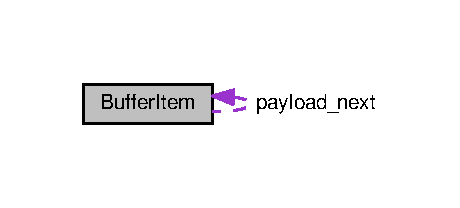
\includegraphics[width=221pt]{structBufferItem__coll__graph}
\end{center}
\end{figure}
\subsection*{Public Attributes}
\begin{DoxyCompactItemize}
\item 
uint8\+\_\+t \hyperlink{structBufferItem_a5c3187c383ceec1825964d5e512273de}{payload\+\_\+size} = 0
\item 
uint8\+\_\+t \hyperlink{structBufferItem_a2e475a18a6671f1f0c4bf3010d7a6e89}{payload\+\_\+destination} = 0
\item 
\hyperlink{structBufferItem}{Buffer\+Item} $\ast$ \hyperlink{structBufferItem_ab20f3ae7cc41c118265557f2c7e2c4f0}{payload\+\_\+next} = 0
\item 
void $\ast$ \hyperlink{structBufferItem_a0ec6d94d7df8c1e9db526fa0200267bb}{payload} = 0
\end{DoxyCompactItemize}


\subsection{Member Data Documentation}
\mbox{\Hypertarget{structBufferItem_a0ec6d94d7df8c1e9db526fa0200267bb}\label{structBufferItem_a0ec6d94d7df8c1e9db526fa0200267bb}} 
\index{Buffer\+Item@{Buffer\+Item}!payload@{payload}}
\index{payload@{payload}!Buffer\+Item@{Buffer\+Item}}
\subsubsection{\texorpdfstring{payload}{payload}}
{\footnotesize\ttfamily void$\ast$ Buffer\+Item\+::payload = 0}

\mbox{\Hypertarget{structBufferItem_a2e475a18a6671f1f0c4bf3010d7a6e89}\label{structBufferItem_a2e475a18a6671f1f0c4bf3010d7a6e89}} 
\index{Buffer\+Item@{Buffer\+Item}!payload\+\_\+destination@{payload\+\_\+destination}}
\index{payload\+\_\+destination@{payload\+\_\+destination}!Buffer\+Item@{Buffer\+Item}}
\subsubsection{\texorpdfstring{payload\+\_\+destination}{payload\_destination}}
{\footnotesize\ttfamily uint8\+\_\+t Buffer\+Item\+::payload\+\_\+destination = 0}

\mbox{\Hypertarget{structBufferItem_ab20f3ae7cc41c118265557f2c7e2c4f0}\label{structBufferItem_ab20f3ae7cc41c118265557f2c7e2c4f0}} 
\index{Buffer\+Item@{Buffer\+Item}!payload\+\_\+next@{payload\+\_\+next}}
\index{payload\+\_\+next@{payload\+\_\+next}!Buffer\+Item@{Buffer\+Item}}
\subsubsection{\texorpdfstring{payload\+\_\+next}{payload\_next}}
{\footnotesize\ttfamily \hyperlink{structBufferItem}{Buffer\+Item}$\ast$ Buffer\+Item\+::payload\+\_\+next = 0}

\mbox{\Hypertarget{structBufferItem_a5c3187c383ceec1825964d5e512273de}\label{structBufferItem_a5c3187c383ceec1825964d5e512273de}} 
\index{Buffer\+Item@{Buffer\+Item}!payload\+\_\+size@{payload\+\_\+size}}
\index{payload\+\_\+size@{payload\+\_\+size}!Buffer\+Item@{Buffer\+Item}}
\subsubsection{\texorpdfstring{payload\+\_\+size}{payload\_size}}
{\footnotesize\ttfamily uint8\+\_\+t Buffer\+Item\+::payload\+\_\+size = 0}



The documentation for this struct was generated from the following file\+:\begin{DoxyCompactItemize}
\item 
\hyperlink{TooNetworking_8h}{Too\+Networking.\+h}\end{DoxyCompactItemize}

\hypertarget{structPayload__Metadata}{}\section{Payload\+\_\+\+Metadata Struct Reference}
\label{structPayload__Metadata}\index{Payload\+\_\+\+Metadata@{Payload\+\_\+\+Metadata}}


{\ttfamily \#include $<$Too\+Networking.\+h$>$}

\subsection*{Public Attributes}
\begin{DoxyCompactItemize}
\item 
uint8\+\_\+t \hyperlink{structPayload__Metadata_a5d517fb1e486f468bef3f42b93b6707d}{payload\+\_\+size} = 0
\end{DoxyCompactItemize}


\subsection{Member Data Documentation}
\mbox{\Hypertarget{structPayload__Metadata_a5d517fb1e486f468bef3f42b93b6707d}\label{structPayload__Metadata_a5d517fb1e486f468bef3f42b93b6707d}} 
\index{Payload\+\_\+\+Metadata@{Payload\+\_\+\+Metadata}!payload\+\_\+size@{payload\+\_\+size}}
\index{payload\+\_\+size@{payload\+\_\+size}!Payload\+\_\+\+Metadata@{Payload\+\_\+\+Metadata}}
\subsubsection{\texorpdfstring{payload\+\_\+size}{payload\_size}}
{\footnotesize\ttfamily uint8\+\_\+t Payload\+\_\+\+Metadata\+::payload\+\_\+size = 0}



The documentation for this struct was generated from the following file\+:\begin{DoxyCompactItemize}
\item 
\hyperlink{TooNetworking_8h}{Too\+Networking.\+h}\end{DoxyCompactItemize}

\chapter{File Documentation}
\hypertarget{TooAutomation_8h}{}\section{Too\+Automation.\+h File Reference}
\label{TooAutomation_8h}\index{Too\+Automation.\+h@{Too\+Automation.\+h}}

\hypertarget{TooNetworking_8h}{}\section{Too\+Networking.\+h File Reference}
\label{TooNetworking_8h}\index{Too\+Networking.\+h@{Too\+Networking.\+h}}
\subsection*{Classes}
\begin{DoxyCompactItemize}
\item 
struct \hyperlink{structBufferItem}{Buffer\+Item}
\item 
struct \hyperlink{structPayload__Metadata}{Payload\+\_\+\+Metadata}
\item 
struct \hyperlink{structPayload__MetadataSigned}{Payload\+\_\+\+Metadata\+Signed}
\item 
struct \hyperlink{structBufferItem__Signed}{Buffer\+Item\+\_\+\+Signed}
\item 
struct \hyperlink{structNonceSent}{Nonce\+Sent}
\item 
struct \hyperlink{structNonceReceived}{Nonce\+Received}
\item 
struct \hyperlink{structNoncePayload}{Nonce\+Payload}
\item 
struct \hyperlink{structNonceRequested}{Nonce\+Requested}
\end{DoxyCompactItemize}
\subsection*{Functions}
\begin{DoxyCompactItemize}
\item 
R\+F24 \hyperlink{TooNetworking_8h_a173f695381b08642c89a68cdcd76a5d4}{radio} (T\+O\+O\+\_\+\+R\+F24\+\_\+\+CE, T\+O\+O\+\_\+\+R\+F24\+\_\+\+CS)
\item 
R\+F24\+Network \hyperlink{TooNetworking_8h_aa7924d94ea32c8d33a81ff41f8678320}{network} (\hyperlink{TooNetworking_8h_a173f695381b08642c89a68cdcd76a5d4}{radio})
\item 
R\+F24\+Mesh \hyperlink{TooNetworking_8h_abdda8f09b9d475ed2c23a2376e2e0151}{mesh} (\hyperlink{TooNetworking_8h_a173f695381b08642c89a68cdcd76a5d4}{radio}, \hyperlink{TooNetworking_8h_aa7924d94ea32c8d33a81ff41f8678320}{network})
\item 
bool \hyperlink{TooNetworking_8h_aec97902cf0d3ec10fd86927f3d1df0c6}{Too\+Networking\+\_\+connection\+\_\+begin} (uint8\+\_\+t passed\+\_\+node\+\_\+id)
\item 
bool \hyperlink{TooNetworking_8h_a723608b997230cc461d06454b2cdb8c3}{Too\+Networking\+\_\+send} (uint8\+\_\+t for\+\_\+node, void $\ast$payload, uint8\+\_\+t size, uint8\+\_\+t type)
\item 
bool \hyperlink{TooNetworking_8h_a9209f3e1a2fdf0b3b88d49105b8fc359}{Too\+Networking\+\_\+send\+\_\+signed} (uint8\+\_\+t for\+\_\+node, void $\ast$payload, uint8\+\_\+t size)
\item 
bool \hyperlink{TooNetworking_8h_a9f893c3218491ee86282fdcd9f376500}{Too\+Networking\+\_\+send\+\_\+signed\+\_\+} (uint8\+\_\+t for\+\_\+node, void $\ast$payload, uint8\+\_\+t size, uint32\+\_\+t nonce)
\item 
bool \hyperlink{TooNetworking_8h_a86fb32acfc42a498be62a3236c778454}{Too\+Networking\+\_\+send\+\_\+encrypted} (uint8\+\_\+t for\+\_\+node, void $\ast$payload, uint8\+\_\+t size)
\item 
bool \hyperlink{TooNetworking_8h_a5861e5d6df60aa6701af1b9ec7e942a8}{Too\+Networking\+\_\+send\+\_\+signed\+\_\+encrypted} (uint8\+\_\+t for\+\_\+node, void $\ast$payload, uint8\+\_\+t size)
\item 
bool \hyperlink{TooNetworking_8h_a8b2b7fde063d7268ae7deabffeba6152}{Too\+Networking\+\_\+peek} (R\+F24\+Network\+Header \&header, void $\ast$message, uint16\+\_\+t maxlen)
\item 
bool \hyperlink{TooNetworking_8h_a9cd17becc197be8de7befa25116c3a67}{Too\+Networking\+\_\+read} (R\+F24\+Network\+Header \&header, void $\ast$message, uint16\+\_\+t maxlen)
\item 
bool \hyperlink{TooNetworking_8h_ac352268e177fa2ddf91c8afa5cd04bbf}{Too\+Networking\+\_\+connection\+\_\+available} ()
\item 
bool \hyperlink{TooNetworking_8h_a48504aef69d9ac92e34269a64f7b518b}{Too\+Networking\+\_\+connection\+\_\+check} ()
\item 
bool \hyperlink{TooNetworking_8h_aefc5dad88b637efb11a3a7b2f76a19b9}{Too\+Networking\+\_\+connection\+\_\+fix} ()
\item 
bool \hyperlink{TooNetworking_8h_a7382ba1aed5405c3adc02011ea6c45dd}{Too\+Networking\+\_\+connection\+\_\+maintenance} ()
\item 
void \hyperlink{group__SIMPLE__BUFFER_ga3c91b7ab2f6500c287ecc7ab4a018ef6}{Too\+Networking\+\_\+bufferlist\+\_\+remove} (\hyperlink{structBufferItem}{Buffer\+Item} $\ast$previous, \hyperlink{structBufferItem}{Buffer\+Item} $\ast$current)
\item 
bool \hyperlink{group__SIMPLE__BUFFER_gaa8a4e879d4d71fed2a8940cf93b75ae4}{Too\+Networking\+\_\+bufferlist\+\_\+initialize} ()
\item 
\hyperlink{structBufferItem}{Buffer\+Item} $\ast$ \hyperlink{group__SIMPLE__BUFFER_ga0dd5e9de81eea99b99669a607c9b4028}{Too\+Networking\+\_\+bufferlist\+\_\+find\+\_\+for\+\_\+id} (uint8\+\_\+t node\+ID)
\item 
bool \hyperlink{group__SIMPLE__BUFFER_gae72372a8084e8486f1306240a9af6474}{Too\+Networking\+\_\+bufferlist\+\_\+send} (\hyperlink{structBufferItem}{Buffer\+Item} $\ast$item, \hyperlink{structNonceReceived}{Nonce\+Received} $\ast$nonce, \hyperlink{structBufferItem}{Buffer\+Item} $\ast$previousitem)
\item 
bool \hyperlink{group__SIMPLE__BUFFER_ga1fca7e85a8a2f91a1b20a8bb23b4e893}{Too\+Networking\+\_\+bufferlist\+\_\+add} (uint8\+\_\+t payload\+\_\+destination, void $\ast$payload, uint8\+\_\+t size)
\item 
void \hyperlink{group__SIMPLE__BUFFER_gab58e06e0eb6f2f8ecbebeaf3c173fb22}{Too\+Networking\+\_\+bufferlist\+\_\+send\+\_\+all} ()
\item 
void \hyperlink{group__SIMPLE__BUFFER_ga2b5485b317146ce7c14bbad26172d796}{Too\+Networking\+\_\+bufferlist\+\_\+print} ()
\item 
bool \hyperlink{TooNetworking_8h_aa9ec1ce0a58a96d0452a5ec51bb0bfca}{Too\+Neteorking\+\_\+connection\+\_\+fix} ()
\item 
bool \hyperlink{TooNetworking_8h_a2676204dee95da1ef337de95eb0e9bcb}{Too\+Networking\+\_\+begin} (uint8\+\_\+t passed\+\_\+node\+\_\+id)
\end{DoxyCompactItemize}
\subsection*{Variables}
\begin{DoxyCompactItemize}
\item 
uint8\+\_\+t \hyperlink{TooNetworking_8h_a4277db94d928ddb590684b5bf9174f73}{current\+\_\+node\+\_\+\+ID}
\item 
Sha256\+Class \hyperlink{TooNetworking_8h_a2cde2cc921aef77784b8d5b3129b5803}{Sha256}
\item 
\hyperlink{structNonceSent}{Nonce\+Sent} $\ast$ \hyperlink{TooNetworking_8h_ae75ffa3e0a98255f366188a6223156bc}{nonce\+\_\+sent\+\_\+start} = 0
\item 
\hyperlink{structNonceReceived}{Nonce\+Received} $\ast$ \hyperlink{TooNetworking_8h_ad145f92b978c39b1728ffd91e896277a}{nonce\+\_\+received\+\_\+start} = 0
\item 
\hyperlink{structNonceRequested}{Nonce\+Requested} $\ast$ \hyperlink{TooNetworking_8h_aac43930ae93d50eea7e1ae8aee603524}{nonce\+\_\+requested\+\_\+first} = 0
\item 
\hyperlink{structBufferItem}{Buffer\+Item} $\ast$ \hyperlink{TooNetworking_8h_a7c24840cd9eb766eb04c1db0d2363cd5}{buffer\+\_\+first} = 0
\end{DoxyCompactItemize}


\subsection{Detailed Description}
This file implements the necessary functionality that allow nodes in the network to communicate 

\subsection{Function Documentation}
\mbox{\Hypertarget{TooNetworking_8h_abdda8f09b9d475ed2c23a2376e2e0151}\label{TooNetworking_8h_abdda8f09b9d475ed2c23a2376e2e0151}} 
\index{Too\+Networking.\+h@{Too\+Networking.\+h}!mesh@{mesh}}
\index{mesh@{mesh}!Too\+Networking.\+h@{Too\+Networking.\+h}}
\subsubsection{\texorpdfstring{mesh()}{mesh()}}
{\footnotesize\ttfamily R\+F24\+Mesh mesh (\begin{DoxyParamCaption}\item[{\hyperlink{TooNetworking_8h_a173f695381b08642c89a68cdcd76a5d4}{radio}}]{,  }\item[{\hyperlink{TooNetworking_8h_aa7924d94ea32c8d33a81ff41f8678320}{network}}]{ }\end{DoxyParamCaption})}

\mbox{\Hypertarget{TooNetworking_8h_aa7924d94ea32c8d33a81ff41f8678320}\label{TooNetworking_8h_aa7924d94ea32c8d33a81ff41f8678320}} 
\index{Too\+Networking.\+h@{Too\+Networking.\+h}!network@{network}}
\index{network@{network}!Too\+Networking.\+h@{Too\+Networking.\+h}}
\subsubsection{\texorpdfstring{network()}{network()}}
{\footnotesize\ttfamily R\+F24\+Network network (\begin{DoxyParamCaption}\item[{\hyperlink{TooNetworking_8h_a173f695381b08642c89a68cdcd76a5d4}{radio}}]{ }\end{DoxyParamCaption})}

\mbox{\Hypertarget{TooNetworking_8h_a173f695381b08642c89a68cdcd76a5d4}\label{TooNetworking_8h_a173f695381b08642c89a68cdcd76a5d4}} 
\index{Too\+Networking.\+h@{Too\+Networking.\+h}!radio@{radio}}
\index{radio@{radio}!Too\+Networking.\+h@{Too\+Networking.\+h}}
\subsubsection{\texorpdfstring{radio()}{radio()}}
{\footnotesize\ttfamily R\+F24 radio (\begin{DoxyParamCaption}\item[{T\+O\+O\+\_\+\+R\+F24\+\_\+\+CE}]{,  }\item[{T\+O\+O\+\_\+\+R\+F24\+\_\+\+CS}]{ }\end{DoxyParamCaption})}

\mbox{\Hypertarget{TooNetworking_8h_aa9ec1ce0a58a96d0452a5ec51bb0bfca}\label{TooNetworking_8h_aa9ec1ce0a58a96d0452a5ec51bb0bfca}} 
\index{Too\+Networking.\+h@{Too\+Networking.\+h}!Too\+Neteorking\+\_\+connection\+\_\+fix@{Too\+Neteorking\+\_\+connection\+\_\+fix}}
\index{Too\+Neteorking\+\_\+connection\+\_\+fix@{Too\+Neteorking\+\_\+connection\+\_\+fix}!Too\+Networking.\+h@{Too\+Networking.\+h}}
\subsubsection{\texorpdfstring{Too\+Neteorking\+\_\+connection\+\_\+fix()}{TooNeteorking\_connection\_fix()}}
{\footnotesize\ttfamily bool Too\+Neteorking\+\_\+connection\+\_\+fix (\begin{DoxyParamCaption}{ }\end{DoxyParamCaption})}

Tries to reestablish connection to the network

\begin{DoxyReturn}{Returns}
True if successful, false otherwise 
\end{DoxyReturn}
\mbox{\Hypertarget{TooNetworking_8h_a2676204dee95da1ef337de95eb0e9bcb}\label{TooNetworking_8h_a2676204dee95da1ef337de95eb0e9bcb}} 
\index{Too\+Networking.\+h@{Too\+Networking.\+h}!Too\+Networking\+\_\+begin@{Too\+Networking\+\_\+begin}}
\index{Too\+Networking\+\_\+begin@{Too\+Networking\+\_\+begin}!Too\+Networking.\+h@{Too\+Networking.\+h}}
\subsubsection{\texorpdfstring{Too\+Networking\+\_\+begin()}{TooNetworking\_begin()}}
{\footnotesize\ttfamily bool Too\+Networking\+\_\+begin (\begin{DoxyParamCaption}\item[{uint8\+\_\+t}]{passed\+\_\+node\+\_\+id }\end{DoxyParamCaption})}

Automatically set up the networking Every radio should provide \hyperlink{TooNetworking_8h_aec97902cf0d3ec10fd86927f3d1df0c6}{Too\+Networking\+\_\+connection\+\_\+begin(uint8\+\_\+t node\+I\+D)} for easy initialization of the network


\begin{DoxyParams}{Parameters}
{\em passed\+\_\+node\+\_\+id} & Current node\textquotesingle{}s ID. \\
\hline
\end{DoxyParams}
\begin{DoxyReturn}{Returns}
true if successful, false otherwise 
\end{DoxyReturn}
\mbox{\Hypertarget{TooNetworking_8h_ac352268e177fa2ddf91c8afa5cd04bbf}\label{TooNetworking_8h_ac352268e177fa2ddf91c8afa5cd04bbf}} 
\index{Too\+Networking.\+h@{Too\+Networking.\+h}!Too\+Networking\+\_\+connection\+\_\+available@{Too\+Networking\+\_\+connection\+\_\+available}}
\index{Too\+Networking\+\_\+connection\+\_\+available@{Too\+Networking\+\_\+connection\+\_\+available}!Too\+Networking.\+h@{Too\+Networking.\+h}}
\subsubsection{\texorpdfstring{Too\+Networking\+\_\+connection\+\_\+available()}{TooNetworking\_connection\_available()}}
{\footnotesize\ttfamily bool Too\+Networking\+\_\+connection\+\_\+available (\begin{DoxyParamCaption}{ }\end{DoxyParamCaption})}

Checks if there\textquotesingle{}s something ready to be processed

\begin{DoxyReturn}{Returns}
True if successful, false otherwise 
\end{DoxyReturn}
\mbox{\Hypertarget{TooNetworking_8h_aec97902cf0d3ec10fd86927f3d1df0c6}\label{TooNetworking_8h_aec97902cf0d3ec10fd86927f3d1df0c6}} 
\index{Too\+Networking.\+h@{Too\+Networking.\+h}!Too\+Networking\+\_\+connection\+\_\+begin@{Too\+Networking\+\_\+connection\+\_\+begin}}
\index{Too\+Networking\+\_\+connection\+\_\+begin@{Too\+Networking\+\_\+connection\+\_\+begin}!Too\+Networking.\+h@{Too\+Networking.\+h}}
\subsubsection{\texorpdfstring{Too\+Networking\+\_\+connection\+\_\+begin()}{TooNetworking\_connection\_begin()}}
{\footnotesize\ttfamily bool Too\+Networking\+\_\+connection\+\_\+begin (\begin{DoxyParamCaption}\item[{uint8\+\_\+t}]{passed\+\_\+node\+\_\+id }\end{DoxyParamCaption})}

Automatically set up the networking, implementation depends on the radio


\begin{DoxyParams}{Parameters}
{\em passed\+\_\+node\+\_\+id} & Current node\textquotesingle{}s ID. \\
\hline
\end{DoxyParams}
\begin{DoxyReturn}{Returns}
true if successful, false otherwise 
\end{DoxyReturn}
\mbox{\Hypertarget{TooNetworking_8h_a48504aef69d9ac92e34269a64f7b518b}\label{TooNetworking_8h_a48504aef69d9ac92e34269a64f7b518b}} 
\index{Too\+Networking.\+h@{Too\+Networking.\+h}!Too\+Networking\+\_\+connection\+\_\+check@{Too\+Networking\+\_\+connection\+\_\+check}}
\index{Too\+Networking\+\_\+connection\+\_\+check@{Too\+Networking\+\_\+connection\+\_\+check}!Too\+Networking.\+h@{Too\+Networking.\+h}}
\subsubsection{\texorpdfstring{Too\+Networking\+\_\+connection\+\_\+check()}{TooNetworking\_connection\_check()}}
{\footnotesize\ttfamily bool Too\+Networking\+\_\+connection\+\_\+check (\begin{DoxyParamCaption}{ }\end{DoxyParamCaption})}

Checks if the master node is reachable

\begin{DoxyReturn}{Returns}
true if successful, false otherwise 
\end{DoxyReturn}
\mbox{\Hypertarget{TooNetworking_8h_aefc5dad88b637efb11a3a7b2f76a19b9}\label{TooNetworking_8h_aefc5dad88b637efb11a3a7b2f76a19b9}} 
\index{Too\+Networking.\+h@{Too\+Networking.\+h}!Too\+Networking\+\_\+connection\+\_\+fix@{Too\+Networking\+\_\+connection\+\_\+fix}}
\index{Too\+Networking\+\_\+connection\+\_\+fix@{Too\+Networking\+\_\+connection\+\_\+fix}!Too\+Networking.\+h@{Too\+Networking.\+h}}
\subsubsection{\texorpdfstring{Too\+Networking\+\_\+connection\+\_\+fix()}{TooNetworking\_connection\_fix()}}
{\footnotesize\ttfamily bool Too\+Networking\+\_\+connection\+\_\+fix (\begin{DoxyParamCaption}{ }\end{DoxyParamCaption})}

Tries to reestablish connection to the network

\begin{DoxyReturn}{Returns}
True if successful, false otherwise 
\end{DoxyReturn}
\mbox{\Hypertarget{TooNetworking_8h_a7382ba1aed5405c3adc02011ea6c45dd}\label{TooNetworking_8h_a7382ba1aed5405c3adc02011ea6c45dd}} 
\index{Too\+Networking.\+h@{Too\+Networking.\+h}!Too\+Networking\+\_\+connection\+\_\+maintenance@{Too\+Networking\+\_\+connection\+\_\+maintenance}}
\index{Too\+Networking\+\_\+connection\+\_\+maintenance@{Too\+Networking\+\_\+connection\+\_\+maintenance}!Too\+Networking.\+h@{Too\+Networking.\+h}}
\subsubsection{\texorpdfstring{Too\+Networking\+\_\+connection\+\_\+maintenance()}{TooNetworking\_connection\_maintenance()}}
{\footnotesize\ttfamily bool Too\+Networking\+\_\+connection\+\_\+maintenance (\begin{DoxyParamCaption}{ }\end{DoxyParamCaption})}

Does the necessary maintenance and D\+H\+CP(-\/like) actions on the network

\begin{DoxyReturn}{Returns}
True if successful, false otherwise
\end{DoxyReturn}
Does the necessary maintenance on the network

\begin{DoxyReturn}{Returns}
True if successful, false otherwise 
\end{DoxyReturn}
\mbox{\Hypertarget{TooNetworking_8h_a8b2b7fde063d7268ae7deabffeba6152}\label{TooNetworking_8h_a8b2b7fde063d7268ae7deabffeba6152}} 
\index{Too\+Networking.\+h@{Too\+Networking.\+h}!Too\+Networking\+\_\+peek@{Too\+Networking\+\_\+peek}}
\index{Too\+Networking\+\_\+peek@{Too\+Networking\+\_\+peek}!Too\+Networking.\+h@{Too\+Networking.\+h}}
\subsubsection{\texorpdfstring{Too\+Networking\+\_\+peek()}{TooNetworking\_peek()}}
{\footnotesize\ttfamily bool Too\+Networking\+\_\+peek (\begin{DoxyParamCaption}\item[{R\+F24\+Network\+Header \&}]{header,  }\item[{void $\ast$}]{message,  }\item[{uint16\+\_\+t}]{maxlen }\end{DoxyParamCaption})}

Allows reading a message from buffer and it\textquotesingle{}s N\+OT cleared after being read


\begin{DoxyParams}{Parameters}
{\em } & \\
\hline
\end{DoxyParams}
\mbox{\Hypertarget{TooNetworking_8h_a9cd17becc197be8de7befa25116c3a67}\label{TooNetworking_8h_a9cd17becc197be8de7befa25116c3a67}} 
\index{Too\+Networking.\+h@{Too\+Networking.\+h}!Too\+Networking\+\_\+read@{Too\+Networking\+\_\+read}}
\index{Too\+Networking\+\_\+read@{Too\+Networking\+\_\+read}!Too\+Networking.\+h@{Too\+Networking.\+h}}
\subsubsection{\texorpdfstring{Too\+Networking\+\_\+read()}{TooNetworking\_read()}}
{\footnotesize\ttfamily bool Too\+Networking\+\_\+read (\begin{DoxyParamCaption}\item[{R\+F24\+Network\+Header \&}]{header,  }\item[{void $\ast$}]{message,  }\item[{uint16\+\_\+t}]{maxlen }\end{DoxyParamCaption})}

Allows reading a message from buffer and it\textquotesingle{}s cleared after being read


\begin{DoxyParams}{Parameters}
{\em } & \\
\hline
\end{DoxyParams}
\mbox{\Hypertarget{TooNetworking_8h_a723608b997230cc461d06454b2cdb8c3}\label{TooNetworking_8h_a723608b997230cc461d06454b2cdb8c3}} 
\index{Too\+Networking.\+h@{Too\+Networking.\+h}!Too\+Networking\+\_\+send@{Too\+Networking\+\_\+send}}
\index{Too\+Networking\+\_\+send@{Too\+Networking\+\_\+send}!Too\+Networking.\+h@{Too\+Networking.\+h}}
\subsubsection{\texorpdfstring{Too\+Networking\+\_\+send()}{TooNetworking\_send()}}
{\footnotesize\ttfamily bool Too\+Networking\+\_\+send (\begin{DoxyParamCaption}\item[{uint8\+\_\+t}]{for\+\_\+node,  }\item[{void $\ast$}]{payload,  }\item[{uint8\+\_\+t}]{size,  }\item[{uint8\+\_\+t}]{type }\end{DoxyParamCaption})}

Allows sending a encrypted message


\begin{DoxyParams}{Parameters}
{\em } & \\
\hline
\end{DoxyParams}
\mbox{\Hypertarget{TooNetworking_8h_a86fb32acfc42a498be62a3236c778454}\label{TooNetworking_8h_a86fb32acfc42a498be62a3236c778454}} 
\index{Too\+Networking.\+h@{Too\+Networking.\+h}!Too\+Networking\+\_\+send\+\_\+encrypted@{Too\+Networking\+\_\+send\+\_\+encrypted}}
\index{Too\+Networking\+\_\+send\+\_\+encrypted@{Too\+Networking\+\_\+send\+\_\+encrypted}!Too\+Networking.\+h@{Too\+Networking.\+h}}
\subsubsection{\texorpdfstring{Too\+Networking\+\_\+send\+\_\+encrypted()}{TooNetworking\_send\_encrypted()}}
{\footnotesize\ttfamily bool Too\+Networking\+\_\+send\+\_\+encrypted (\begin{DoxyParamCaption}\item[{uint8\+\_\+t}]{for\+\_\+node,  }\item[{void $\ast$}]{payload,  }\item[{uint8\+\_\+t}]{size }\end{DoxyParamCaption})}

Allows sending an encrypted message


\begin{DoxyParams}{Parameters}
{\em } & \\
\hline
\end{DoxyParams}
\mbox{\Hypertarget{TooNetworking_8h_a9209f3e1a2fdf0b3b88d49105b8fc359}\label{TooNetworking_8h_a9209f3e1a2fdf0b3b88d49105b8fc359}} 
\index{Too\+Networking.\+h@{Too\+Networking.\+h}!Too\+Networking\+\_\+send\+\_\+signed@{Too\+Networking\+\_\+send\+\_\+signed}}
\index{Too\+Networking\+\_\+send\+\_\+signed@{Too\+Networking\+\_\+send\+\_\+signed}!Too\+Networking.\+h@{Too\+Networking.\+h}}
\subsubsection{\texorpdfstring{Too\+Networking\+\_\+send\+\_\+signed()}{TooNetworking\_send\_signed()}}
{\footnotesize\ttfamily bool Too\+Networking\+\_\+send\+\_\+signed (\begin{DoxyParamCaption}\item[{uint8\+\_\+t}]{for\+\_\+node,  }\item[{void $\ast$}]{payload,  }\item[{uint8\+\_\+t}]{size }\end{DoxyParamCaption})}

Allows sending a signed message, type must be embedded inside the payload the receiver must know what to do with the message once it\textquotesingle{}s been verified, messages that fail the checks are D\+I\+S\+C\+A\+R\+D\+E\+D!


\begin{DoxyParams}{Parameters}
{\em for\+\_\+node} & destination \\
\hline
{\em payload} & payload \\
\hline
{\em size} & size of payload \\
\hline
\end{DoxyParams}
\begin{DoxyReturn}{Returns}
true if successful, false otherwise 
\end{DoxyReturn}
\mbox{\Hypertarget{TooNetworking_8h_a9f893c3218491ee86282fdcd9f376500}\label{TooNetworking_8h_a9f893c3218491ee86282fdcd9f376500}} 
\index{Too\+Networking.\+h@{Too\+Networking.\+h}!Too\+Networking\+\_\+send\+\_\+signed\+\_\+@{Too\+Networking\+\_\+send\+\_\+signed\+\_\+}}
\index{Too\+Networking\+\_\+send\+\_\+signed\+\_\+@{Too\+Networking\+\_\+send\+\_\+signed\+\_\+}!Too\+Networking.\+h@{Too\+Networking.\+h}}
\subsubsection{\texorpdfstring{Too\+Networking\+\_\+send\+\_\+signed\+\_\+()}{TooNetworking\_send\_signed\_()}}
{\footnotesize\ttfamily bool Too\+Networking\+\_\+send\+\_\+signed\+\_\+ (\begin{DoxyParamCaption}\item[{uint8\+\_\+t}]{for\+\_\+node,  }\item[{void $\ast$}]{payload,  }\item[{uint8\+\_\+t}]{size,  }\item[{uint32\+\_\+t}]{nonce }\end{DoxyParamCaption})}

Allows sending a signed message, type must be embedded inside the payload the receiver must know what to do with the message once it\textquotesingle{}s been verified, messages that fail the checks are D\+I\+S\+C\+A\+R\+D\+E\+D!


\begin{DoxyParams}{Parameters}
{\em for\+\_\+node} & destination \\
\hline
{\em payload} & payload \\
\hline
{\em size} & size of payload \\
\hline
{\em nonce} & nonce \\
\hline
\end{DoxyParams}
\begin{DoxyReturn}{Returns}
true if successful, false otherwise 
\end{DoxyReturn}
\mbox{\Hypertarget{TooNetworking_8h_a5861e5d6df60aa6701af1b9ec7e942a8}\label{TooNetworking_8h_a5861e5d6df60aa6701af1b9ec7e942a8}} 
\index{Too\+Networking.\+h@{Too\+Networking.\+h}!Too\+Networking\+\_\+send\+\_\+signed\+\_\+encrypted@{Too\+Networking\+\_\+send\+\_\+signed\+\_\+encrypted}}
\index{Too\+Networking\+\_\+send\+\_\+signed\+\_\+encrypted@{Too\+Networking\+\_\+send\+\_\+signed\+\_\+encrypted}!Too\+Networking.\+h@{Too\+Networking.\+h}}
\subsubsection{\texorpdfstring{Too\+Networking\+\_\+send\+\_\+signed\+\_\+encrypted()}{TooNetworking\_send\_signed\_encrypted()}}
{\footnotesize\ttfamily bool Too\+Networking\+\_\+send\+\_\+signed\+\_\+encrypted (\begin{DoxyParamCaption}\item[{uint8\+\_\+t}]{for\+\_\+node,  }\item[{void $\ast$}]{payload,  }\item[{uint8\+\_\+t}]{size }\end{DoxyParamCaption})}

Allows sending a signed and encrypted message


\begin{DoxyParams}{Parameters}
{\em } & \\
\hline
\end{DoxyParams}


\subsection{Variable Documentation}
\mbox{\Hypertarget{TooNetworking_8h_a7c24840cd9eb766eb04c1db0d2363cd5}\label{TooNetworking_8h_a7c24840cd9eb766eb04c1db0d2363cd5}} 
\index{Too\+Networking.\+h@{Too\+Networking.\+h}!buffer\+\_\+first@{buffer\+\_\+first}}
\index{buffer\+\_\+first@{buffer\+\_\+first}!Too\+Networking.\+h@{Too\+Networking.\+h}}
\subsubsection{\texorpdfstring{buffer\+\_\+first}{buffer\_first}}
{\footnotesize\ttfamily \hyperlink{structBufferItem}{Buffer\+Item} $\ast$ buffer\+\_\+first = 0}

Pointer to the payload list start \mbox{\Hypertarget{TooNetworking_8h_a4277db94d928ddb590684b5bf9174f73}\label{TooNetworking_8h_a4277db94d928ddb590684b5bf9174f73}} 
\index{Too\+Networking.\+h@{Too\+Networking.\+h}!current\+\_\+node\+\_\+\+ID@{current\+\_\+node\+\_\+\+ID}}
\index{current\+\_\+node\+\_\+\+ID@{current\+\_\+node\+\_\+\+ID}!Too\+Networking.\+h@{Too\+Networking.\+h}}
\subsubsection{\texorpdfstring{current\+\_\+node\+\_\+\+ID}{current\_node\_ID}}
{\footnotesize\ttfamily uint8\+\_\+t current\+\_\+node\+\_\+\+ID}

\mbox{\Hypertarget{TooNetworking_8h_ad145f92b978c39b1728ffd91e896277a}\label{TooNetworking_8h_ad145f92b978c39b1728ffd91e896277a}} 
\index{Too\+Networking.\+h@{Too\+Networking.\+h}!nonce\+\_\+received\+\_\+start@{nonce\+\_\+received\+\_\+start}}
\index{nonce\+\_\+received\+\_\+start@{nonce\+\_\+received\+\_\+start}!Too\+Networking.\+h@{Too\+Networking.\+h}}
\subsubsection{\texorpdfstring{nonce\+\_\+received\+\_\+start}{nonce\_received\_start}}
{\footnotesize\ttfamily \hyperlink{structNonceReceived}{Nonce\+Received}$\ast$ nonce\+\_\+received\+\_\+start = 0}

Pointer to the received nonce list start \mbox{\Hypertarget{TooNetworking_8h_aac43930ae93d50eea7e1ae8aee603524}\label{TooNetworking_8h_aac43930ae93d50eea7e1ae8aee603524}} 
\index{Too\+Networking.\+h@{Too\+Networking.\+h}!nonce\+\_\+requested\+\_\+first@{nonce\+\_\+requested\+\_\+first}}
\index{nonce\+\_\+requested\+\_\+first@{nonce\+\_\+requested\+\_\+first}!Too\+Networking.\+h@{Too\+Networking.\+h}}
\subsubsection{\texorpdfstring{nonce\+\_\+requested\+\_\+first}{nonce\_requested\_first}}
{\footnotesize\ttfamily \hyperlink{structNonceRequested}{Nonce\+Requested}$\ast$ nonce\+\_\+requested\+\_\+first = 0}

Pointer to the requested nonce list start \mbox{\Hypertarget{TooNetworking_8h_ae75ffa3e0a98255f366188a6223156bc}\label{TooNetworking_8h_ae75ffa3e0a98255f366188a6223156bc}} 
\index{Too\+Networking.\+h@{Too\+Networking.\+h}!nonce\+\_\+sent\+\_\+start@{nonce\+\_\+sent\+\_\+start}}
\index{nonce\+\_\+sent\+\_\+start@{nonce\+\_\+sent\+\_\+start}!Too\+Networking.\+h@{Too\+Networking.\+h}}
\subsubsection{\texorpdfstring{nonce\+\_\+sent\+\_\+start}{nonce\_sent\_start}}
{\footnotesize\ttfamily \hyperlink{structNonceSent}{Nonce\+Sent}$\ast$ nonce\+\_\+sent\+\_\+start = 0}

Pointer to the sent nonce list start \mbox{\Hypertarget{TooNetworking_8h_a2cde2cc921aef77784b8d5b3129b5803}\label{TooNetworking_8h_a2cde2cc921aef77784b8d5b3129b5803}} 
\index{Too\+Networking.\+h@{Too\+Networking.\+h}!Sha256@{Sha256}}
\index{Sha256@{Sha256}!Too\+Networking.\+h@{Too\+Networking.\+h}}
\subsubsection{\texorpdfstring{Sha256}{Sha256}}
{\footnotesize\ttfamily Sha256\+Class Sha256}

Hashing library object construction 
\hypertarget{TooSensors_8h}{}\section{Too\+Sensors.\+h File Reference}
\label{TooSensors_8h}\index{Too\+Sensors.\+h@{Too\+Sensors.\+h}}


\subsection{Detailed Description}
This file implements the necessary functionality that allow nodes to capture and send data 
%--- End generated contents ---

% Index
\backmatter
\newpage
\phantomsection
\clearemptydoublepage
\addcontentsline{toc}{chapter}{Index}
\printindex

\end{document}
